\documentclass[10pt,a4paper]{article}
\usepackage[utf8]{inputenc} % para poder usar tildes en archivos UTF-8
\usepackage[spanish]{babel} % para que comandos como \today den el resultado en castellano
\usepackage{fullpage} %small margins
\usepackage[parfill]{parskip} %genera saltos entre parrafos
\usepackage{color}
\definecolor{gray}{gray}{0.35}
\usepackage{listings}
\usepackage{enumitem}
\usepackage{amsmath} %big brackets
\lstset{
    numbers=left,
    breaklines=true,
    tabsize=2,
    basicstyle=\ttfamily\color{gray},
}
\setlength{\parindent}{8pt}
\usepackage{mathtools}
\usepackage[margin=50pt]{geometry}
\usepackage{amsfonts}
\usepackage{flafter}
\usepackage{multicol}
\usepackage{subcaption}

\begin{document}

\section{Heurística de búsqueda local}
\subsection{Desarrollo}
\noindent \textbf{\underline{Comentarios preliminares}}
\hfill \newline
\begin{itemize}
\item Si bien es cierto que para los conjuntos, como elementos matemáticos, no es coherente que exista una ''posición'' dentro de ellos, en otras palabras, una noción de orden de los elementos de los mismo, voy a asumir que hay una asignación implícita que está atada a la distribución de los nodos descripta por la solución. Es decir, un nodo tiene asignado un número $x$ en la solución $\iff$ el conjunto, dentro de la particion, al que pertenece se etiqueta como $x$.
\item El pseudo-código descripto más abajo es de bastante alto nivel para luego facilitar la lectura del código fuente.
\item El cálculo de los valores de ciertos índices (por ej: en qué conjunto estoy, en qué posición del vector estoy, entre otros) se realiza inmediatamente luego de entrar al while principal, en ambas vecindades. Se programó así para que haya menos código y sea más simple a la vista.
\item Solucion es un vector de ints, Grafo es una matriz de Peso, Peso es float, Particion es vector de vectores de nodos. 
\end{itemize}
\hfill \newline
\textbf{\underline{Formalización de vecindades y pseudo-códigos}}
\hfill \newline

\textbf{Heurística de Búsqueda Local 1}

La vecindad, en este caso, va a estar definida por $N(S, numConjActual, posConjActual) = $ intercambiar, en la partición formada por $S$ que denotamos como $particionSolucion$, el nodo que corresponde al conjunto $numConjActual$ en la ''posición'' $posConjActual$ por algún otro nodo de conjuntos, de la misma partición, $numConjComparar$ tales que $numConjActual < numConjComparar$; \newline con $1 \leq numConjActual < numConjComparar \leq k$, $1 \leq posConjActual \leq \#(conjActual)$. 

Para ilustrar parte de la idea:

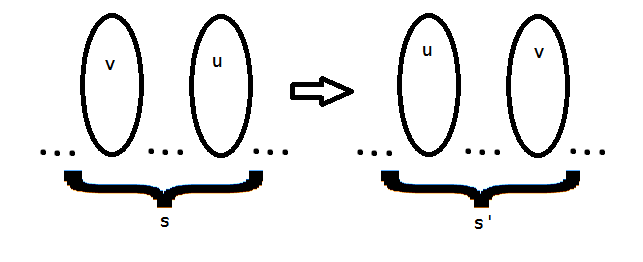
\includegraphics[scale=0.75]{Vecindad1.png}

Por ende, lo que debe hacer el algoritmo es, dada la ubicación actual $(numConjActual, posConjActual)$, debe buscar en los conjuntos, cuyas ''posiciones'' relativas a la particion son $\{(numConjActual+1)...k\}$, algún nodo que al intercambiarlo mejore el peso total de la partición. En otras palabras, un conjunto dentro de la partición tal que $conjActual'$ y $conjComparar'$, que son los conjunto resultado luego de intercambiar el nodo de $numConjActual$ en $posConjActual$ con algún nodo perteneciente a $conjComparar$, cumplan la siguiente desigualdad $peso(conjActual) + peso(conjComparar) > peso(conjActual') + peso(conjComparar')$.

Notar 2 detalles:

\begin{itemize}
\item No se busca intercambios en el mismo conjunto ya que el peso resultaría idéntico.
\item El último conjunto a explorar en busca de intercambios es el $k$, ya que no hay conjuntos ''delante'' del $k$.
\end{itemize}

\hfill \newpage
\textbf{Pseudo-código}

\begin{lstlisting}
busqueda_local_1(Solucion solucion, Int k, Grafo grafo)
	Particion particionSolucion(k)
	organizar los nodos en particionSolucion acorde a solucion

	si k > 1
		numConjActual = 0
		numConjComparar = 1
		posConjActual = 0
		posConjComparar = 0
		
		mientras numConjActual < k
			si (termine de recorrer el conjunto actual)
				buscar en (numConActual+1...k) el proximo conjunto no vacio y colocar su numero en numConjActual
				
				si numConjActual < k
					buscar en (numConjActual+1...k) el proximo conjunto no vacio y colocar su numero en numConjComparar
					
					si numConjComparar > k
						terminar ejecucion
					fin si
					
					posConjActual = 0
				si no
					terminar ejecucion
				fin si
			fin si
			
			si (termine de recorrer el conjunto comparar)
				buscar en (numConjComparar+1...k) el proximo conjunto no vacio y colocar su numero en numConjComparar
				
				si numConjComparar > k
					posConjActual++
					buscar en (numConjActual+1...k) el proximo conjunto no vacio y colocar su numero en numConjComparar
					
					si numConjComparar > k
						terminar ejecucion
					fin si
				fin si
			fin si
			
			posConjComparar = 0
			
			mientras ((no termine de recorrer conjActual) && (no termine de recorrer conjComparar))
				pesoConjActual = peso(particionSolucion[numConjActual], grafo)
				pesoConjComparar = peso(particionSolucion[numConjComparar], grafo)
				hago swap de los nodos
				pesoConjActualMod = peso(particionSolucion[numConjActual], grafo)
				pesoConjCompararMod = peso(particionSolucion[numConjComparar], grafo)
				si (pesoConjActual + pesoConjComparar <= pesoConjActualMod + pesoConjCompararMod)
					deshago el swap y coloco los nodos en sus conjuntos originales
					posConjComparar++
				si no
					modifico solucion con los valores acordes
					posConjComparar++
					posConjActual++
				fin si
			fin mientras
		fin mientras
	fin si
fin funcion
\end{lstlisting}

\textbf{Heurística de Búsqueda Local 2}

La segunda vecindad está sujeta a la siguiente relación, $N(S) = $ quitar un nodo de un conjunto de la particion y colocarlo en otro conjunto de la misma particion. En este caso, no estoy tomando 2 nodos particulares, sino estoy observando el comportamiento de 1 sólo nodo, puesto en otros conjuntos.

Dicho esto, un vecino que mejore el peso total de la solución es aquel tal que quito un nodo de un conjunto, denominado $conjActual$, y lo coloco en otro conjunto, distinguido como $conjAgregar$, tal que el resultado de ese cambio, resultando en $conjActual'$ y $conjAgregar'$, se comporte de acuerdo a la siguiente desigualdad: $peso(conjActual) + peso(conjComparar) > peso(conjActual') + peso(conjComparar')$.

Notar que:

\begin{itemize}
\item Cada vez que encuentro un vecino favorable, que mejore el peso total, debo volver a revisar desde el ''principio'' toda la partición, ya que mi vecindad pide existencia en toda la partición, no desde un conjunto en adelante como la anterior.
\end{itemize}

\textbf{Pseudo-código}

\begin{lstlisting}
void busqueda_local_2(Solucion solucion, int k, Grafo grafo)
	Particion particionSolucion(k)
	organizar los nodos en particionSolucion acorde a solucion
	
	si k > 1
		numConjComparar = 1
		numConjActual = 0
		posConjActual = 0
		
		mientras (numConjActual < k + 1)
			si (termine de recorrer el conjActual)
				buscar en (numConActual+1...k) el proximo conjunto no vacio y colocar su numero en numConjActual
				posDentroConjActual = 0;				
				
				si (numConjActual > k)
					terminar ejecucion
				si no
					numConjComparar = ((numConjActual == 0) ? 1 : 0)
				fin si
			fin si
			
			mientras (numConjAgregar < k)
				pesoConjActual = peso(particionSolucion[numConjActual], grafo)
				pesoConjAgregar = peso(particionSolucion[numConjAgregar], grafo)
				pesoConjActualMod = pesoConjActual - pesoDeNodoEnConjunto(particionSolucion[numConjActual], nodo actual, grafo)
				pesoConjCompararMod = pesoConjComparar + pesoDeNodoEnConjunto(particionSolucion[numConjAgregar], nodo actual, grafo)
				
				si(pesoConjActual + pesoConjAgregar <= pesoConjActualMod + pesoConjAgregarMod)
					numConjAgregar++
					si numConjAgregar == numConjActual
						numConjAgregar++
					fin si
				si no
					quitar nodo actual de conjunto actual
					colocar nodo actual en conjunto agregar
					modifico solucion con los valores acordes
					
					posConjActual = 0
					buscar en (1...k) el proximo conjunto no vacio y colocar su numero en numConjActual
					
					numConjComparar = ((numConjActual == 0) ? 1 : 0)
				fin si
			fin mientras
			
			posConjActual++
		fin mientras
	fin si
fin funcion
\end{lstlisting}
\newpage

\subsection{Complejidad}
\noindent \textbf{\underline{Comentarios preliminares}}
\begin{itemize}
\item Vector es la estructura de la librería STL de C++, con las correspondientes complejidades para sus operaciones. Los valores float e int, son los provistos, nativamente, por el lenguaje. Definimos: Peso como float, Nodo como int, Grafo como vector(vector(Peso)), conjNodos como vector(Nodo), Partición como vector(conjNodos) y Solución como vector(int).
\item Como referencia, usamos el código fuente que se encuentra al final del documento.
\item Consideramos la línea 1 de cada función como la declaración de la misma (return type, parametros y apertura de llaves). Por ende, cuando se mencione ''el código en la línea x'', se está haciendo referencia al código que se encuentra en la línea x desde la línea 1.
\item Operaciones triviales (pedir el tamaño de un vector, comparaciones entre ints, etc) no van a ser mencionadas en el cálculo de complejidad, excepto en casos donde no sea evidente que tienen la complejidad que declaramos.
\end{itemize}

\noindent \textbf{\underline{Complejidad Algoritmo de Búsqueda Local 1}}

Es posible dar una cota de complejidad del algoritmo ya que la vecindad está definida no sólo en base a la solución, sino también por el conjunto y el nodo que estoy analizando actualmente. En palabras más formales, el tamaño de la vecindad se va reduciendo a medida que el algoritmo encuentra un vecino ''mejor''.

\begin{itemize}
\item Línea 4: Declaración particiónSolución con tamaño k $\in \Theta(k)$
\item Líneas 5 - 7: for de $0$ a $(k-1)$ que hace operación reserve con parámetro $n$, la operación reserve $\in O(n)$, entonces el for $\in O(k*n)$
\item Líneas 9 - 10: for de $0$ a $(n-1)$ que hace push\_back al conjunto dentro de la partición correspondiente, el operator[] $\in O(1)$ mientras que, por haber hecho reserve($n$) previamente, push\_back $\in O(1)$. Complejidad total = $O(n)$.
\item Línea 14 - 23: Declaraciones de ints y floats, y a su vez uso de operación .size(). En conjunto, las operaciones $\in O(1)$.
\item Línea 26 - 96: While que ejecuta su cuerpo $(k-1)$ veces $\in \Theta(k*CuerpoWhile1)$.
\item CuerpoWhile1:
\begin{itemize}
\item Líneas 30 - 32: While que itera $k$ veces, en peor caso, realizando operaciones con complejidad $\in O(1)$ $\Rightarrow \in O(k)$.
\item Líneas 37 - 39: While que itera $k$ veces, en peor caso, realizando operaciones con complejidad $\in O(1)$ $\Rightarrow \in O(k)$.
\item Líneas 53 - 55: While que itera $k$ veces, en peor caso, realizando operaciones con complejidad $\in O(1)$ $\Rightarrow \in O(k)$.
\item Líneas 63 - 64: While que itera $k$ veces, en peor caso, realizando operaciones con complejidad $\in O(1)$ $\Rightarrow \in O(k)$.
\item Líneas 75 - 93: While que ejecuta su cuerpo tantas veces como cantidad de elementos haya en conjComparar y conjActual, cuyos tamaños están acotados por $n \Rightarrow \in O(2n*CuerpoWhile2) = O(n*CuerpoWhile2)$.
\item CuerpoWhile2:
\begin{itemize}
\item Líneas 76 - 81: 4 Operaciones pesoDeConjunto, que $\in O(n^2)$ (ver Complejidad Algoritmos Usados), más complejidad del swap $O(1)$ (ver Complejidad Algoritmos Usados) $\Rightarrow O(4*n^2) + O(1) = O(n^2)$.
\item Líneas 83 - 93: Cualquiera de los 2 caminos del if tiene complejidad $O(1)$.
\item Complejidad Total CuerpoWhile2 $\in O(n^2)$.
\end{itemize}
\item Complejidad Total CuerpoWhile1 $\in O(4k + n*(n^2)) = O(k + n^3)$.
\end{itemize}
\end{itemize}

La función que caracteriza la complejidad del algoritmo $\in O(k*n + n + k*(k + n^3)) = O(k*n + k^2 + n^3) = O(k^2 * n^3)$.

\newpage
\noindent \underline{\textbf{Complejidad Iteración Algoritmo de Búsqueda Local 2}}

Para este algoritmo, el análisis de complejidad va a estar sujeto a una iteración del ciclo principal (Líneas 23 - 74) del mismo ya que no hay una cota clara en cuanto a la cantidad de iteraciones del mismo. Una vez que encuentro un conjunto tal que poniendo el nodo actual mejoro el peso total, debo volver a recorrer todos los conjuntos. En otras palabras, la vecindad, dada por el 2do algoritmo de búsqueda local, es más amplia que el primero y no sufre disminuciones en su tamaño.

\begin{itemize}
\item Líneas 26 - 28: While que itera $k$ veces, en peor caso, realizando operaciones con complejidad $\in O(1)$ $\Rightarrow \in O(k)$.
\item Líneas 44 - 45: 2 Operaciones pesoDeConjunto, que $\in O(n^2)$ (ver Complejidad Algoritmos Usados) $\Rightarrow O(2*n^2) = O(n^2)$.
\item Líneas 46 - 47: 2 Operaciones pesoDeNodoEnConjunto, que $\in O(n)$ (ver Complejidad Algoritmos Usados) $\Rightarrow O(2*n) = O(n)$.
\item Línea 56: Operación push\_back() y operator[], ambos con complejidad O(1), complejidad de la línea $\in O(1)$.
\item Línea 57: Operación erase() tiene complejidad lineal en la cantidad de elementos que hay en las posiciones siguientes al último elemento borrado, el peor caso es borrar el primero, $\Rightarrow \in O(n)$ (si para mover los elementos realiza copias, no hay problema ya que copiar ints es $O(1)$).
\item Línea 63 - 65: While que itera $k$ veces, en peor caso, realizando operaciones con complejidad $\in O(1)$ $\Rightarrow \in O(k)$.
\end{itemize}

Habiendo analizado todo lo relevante, en cuánto a complejidad temporal, del código, observamos que la función que caracteriza la complejidad de una iteración del ciclo principal $\in O(2k + (n^2) + n) = O(k + n^2)$.

\textbf{Complejidad Algoritmos Usados}

\underline{pesoDeSolucion}

Función que, dada una solución, un valor k y su Grafo asociado, devuelve un valor que representa el peso de esa solución.

\begin{itemize}
\item Línea 3: Declaración particiónSolución con tamaño k $\in \Theta(k)$.
\item Línea 4 - 5: for de $0$ a $(k-1)$ que hace operación reserve con parámetro $n$, la operación reserve $\in O(n)$, entonces el for $\in O(k*n)$.
\item Línea 7 - 8: for de $0$ a $(n-1)$ que hace push\_back al conjunto dentro de la partición correspondiente, el operator[] $\in O(1)$ mientras que, por haber hecho reserve($n$) previamente, push\_back $\in O(1)$. Complejidad total = $O(n)$.
\item Línea 10: $O(f(n))$, donde $f(n)$ representa la función de complejidad de la función pesoDePartición $\Rightarrow \in O(f(n)) = O(k*n^2)$.
\end{itemize}

Por ende, la complejidad total pertenece al orden de $O(k + k*n + n + k*n^2) = O(k*n^2)$, donde $n$ es la cantidad de nodos en la solución.

\underline{pesoDePartición}

Función que, dada una partición de nodos y el Grafo que corresponda a dichos nodos, nos devuelve un valor que representa el peso de esa partición.

\begin{itemize}
\item Línea 2 - 3: un for de k iteraciones que llama a pesoDeConjunto y suma a acum el valor devuelto. Si llamamos g(n) a la función que describe la complejidad temporal de la función pesoDeConjunto $\Rightarrow \in O(k*g(n)) + O(1) = O(k*O(n^2)) + O(1) = O(k*n^2)$, ya que, en peor caso, un conjunto tiene tamaño $n$, todos los elementos.
\end{itemize}

La complejidad total de esta función $\in O(k*n^2)$, donde $n$ es la cantidad de nodos en la partición.

\underline{pesoDeConjunto}

Función que, dado un conjunto de nodos y Grafo asociado a ellos, nos otorga el peso total de dicho conjunto.

\begin{itemize}
\item Línea 4: for desde $0$ hasta $(n-1)$ $\Rightarrow \in O(n*CuerpoFor)$
\item CuerpoFor:
\begin{itemize}
\item Línea 5: for que itera desde $i$ hasta $(n-1)$ realizando operaciones con costo temporal $O(1)$. El peor caso es $i = 0$ ya que de esa forma itera mayor cantidad de veces $\Rightarrow \in O(n)*O(1) = O(n)$.
\end{itemize}
\item Complejidad Total CuerpoFor $\in O(n^2)$
\end{itemize}

La complejidad total de pesoDeConjunto es de orden cuadrático en $n$, siendo $n$ la cantidad de elementos del conjunto.

\underline{swapEnParticion}

Función que, dado una partición y la posición de 2 nodos en dicha partición, intercambia los lugares de ellos.

\begin{itemize}
\item Líneas 2 - 4: Operaciones de creación y asignación de ints y uso de operator[], todas operaciones con costo temporal constante.
\end{itemize}

Complejidad total de swapEnParticion $\in O(1)$.

\underline{pesoDeNodoEnConjunto}

Función que, dado un nodo, un conjunto de nodos y su Grafo asociado, nos indica la suma de las aristas de los vecinos de dicho nodo en el conjunto. Cabe aclarar que el nodo puede o no pertenecer al conjunto previo a su ejecución.

\begin{itemize}
\item Líneas 4 - 6: for que itera tantas veces como elementos haya en él, cuyo peor caso es $n$, realizando operaciones con costo costante $\Rightarrow \in O(n)$.
\end{itemize}

Complejidad total de pesoDeNodoEnConjunto $\in O(n)$.

\newpage
\subsection{Experimentación}
\noindent \textbf{\underline{Comentarios preliminares}}

La razón detrás de la poca cantidad de análisis de calidad es que resolver instancias con el algoritmo exacto, para obtener valores de solución óptimos, comienza a ser excesivamente demandante en tiempo. Nos pareció que con la cantidad provista de instancias se puede observar el comportamiento argumentado.

\noindent \textbf{\underline{Análisis de calidad}}

\textbf{Casos Relevantes}

¿A qué llamamos casos relevantes? Lo casos relevantes consideramos que son instancias tales que $k < n$. Esto se debe a que, si $k \geq n$, tenemos un algoritmo exacto con complejidad temporal que resuelve el problema, el algoritmo de la heurística golosa. Podríamos no usar dicho algoritmo y armar uno que haga lo siguiente: sabiendo que $k \geq n$ (se pregunta si $k \geq n$ luego de tomar el input), ponemos un nodo por conjunto, y sabemos que eso nos entrega una solución con pesos total igual a $0$ ya que todos los conjuntos contienen un solo valor.
Siguiendo esta lógica, los análisis de calidad están sujetos a estas condiciones. No es el caso de los análisis de complejidad (explicado más adelante).

\textbf{Gráficos}

Para cada instanciaa, tomamos una solución obtenida del algoritmo de heurística golosa y una solución aleatoria. Luego, en base a cada solución, corríamos las heurísticas de búsqueda local y observamos los resultados.

\begin{figure}[h]
        \begin{subfigure}[b]{0.5\textwidth}
                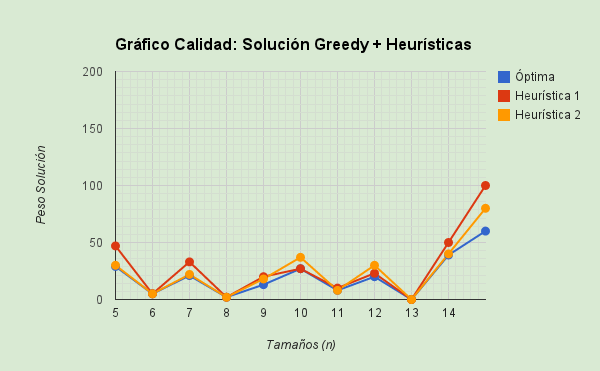
\includegraphics[width=\textwidth]{grafico_calidad_greedy_heurisitcas.png}
        \end{subfigure}
        \begin{subfigure}[b]{0.5\textwidth}
                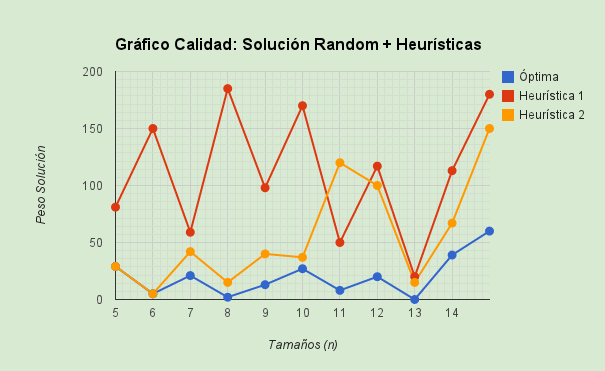
\includegraphics[width=\textwidth]{grafico_calidad_random_heurisitcas.png}
        \end{subfigure}
\end{figure}

\textbf{Conclusiones del análisis de calidad}

Primero que todo, se cumplió algo que es bastante lógico (pero que puede no ser cierto para todo problema ni para toda instancia de este problema): Es preferible tener una solución golosa que una totalmente aleatoria. En términos técnicos, lo que sucede es que la vecindad de la solución aleatoria, en general, "es peor" que la vecindad de una solución relativamente púlida, como la golosa. Esto no necesariamente implica que los vecinos de una solución golosa sean siempre mejores. Un caso en el que no ocurre es el siguiente, un Grafo con $n$ ($n \geq 2$, para que pueda tener al menos una arista) nodos donde todas sus aristas tenga peso $0$, excepto una que tiene peso $p$. Si ocurre que la solución random tiene peso $p$, cualquier heurística nuestra sea, va a tener en su vecindad a la óptima (basta con mover uno de los 2 nodos a otro conjunto o intercambiarlo con algún otro, excepto en que esté en el conjunto k, para la búsqueda local 1). La vecindad sigue siendo peor, pero entre sus vecinos va a tener al óptimo.\newline
\indent Pero ese no es el único detalle interesante. Observemos que, en lineas generales, el algoritmo de busqueda local 2 obtiene mejores soluciones. Esto contradice lo que inicialmente habíamos pensado, ya que la heurística local 1 realiza una búsqueda más exhaustiva.

\newpage
\noindent \textbf{\underline{Análisis de Tiempos}}

\textbf{Casos analizados}

Las instancias para este análisis no cumplen, necesariamente, la desigualdad $k \geq n$ como era el caso para el análisis de calidad. La diferencia es que $k$ aporta para la complejidad temporal y no es algo que podamos pasar por alto. En el caso previo, tener un $k$ muy alto no contribuye en nada ya que agregaría conjuntos vacíos que nada sumarían al valor total de una solución.

\textbf{Gráfico}

Estas mediciones es que los algoritmos fueron corridos en base a una solución aleatoria ya que, de otra forma, se podría condicionar la velocidad de los algoritmos, ya sea para mejor o para peor. El procedimiento se basó en generar 100 instancias de cada tamaño, realizar 50 mediciones de tiempo de cada una y tomar la que menor tiempo tomó, y luego sobre las 100 mediciones tomar un promedio, obteniendo un número que representa coherentemente la generalidad de instancias. Decidimos tomar el menor tiempo de cada instancia ya que representa más fielmente lo que tomaría para ella, debido a que eliminamos tiempo en el que el procesador puede estar atendiendo otros procedimientos y/o operaciones que nada tienen que ver con la ejecución del algoritmo.

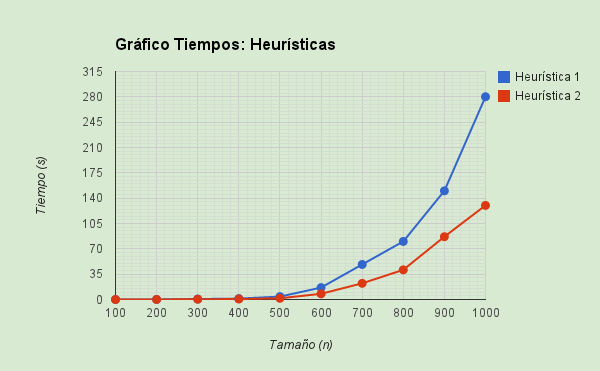
\includegraphics[scale=0.5]{grafico_tiempos_heuristicas.png}

\textbf{Conclusiones del análisis de tiempos}

En base a estos gráficos podemos concluir que el algoritmo de búsqueda local 2 es mejor que el 1. No solo nos brinda mejores soluciones sino que también lo hace más rápido.
En cuánto a la relación con la complejidad temporal se puede ver que ninguna crece de manera exponencial, más bien polinomial, pero si que el algoritmo de búsqueda local 1 crece con mucha más violencia que el otro. Esto nos dice que comparar 2 algoritmos uno con cota de complejidad definida y otro con una no tan claram que resuelvan el mismo problema, no siempre resulta que el que no posee la cota sea "peor".

\noindent \underline{\textbf{Comentarios finales}}

La idea detrás de ambos algoritmos fue que uno de los 2 sea más pesado y exhaustivo, con una vecindad más amplia, de forma tal que otorgue mejores resultados. Lo ocurrido, en lineas generales, no fue eso. El algoritmo 1 termino por vencer, en ambos sentidos, al 2. Eso nos da la pauta de mayor vecindad no siempre implica mejores resultados.
\end{document}